% CS F407 Artificial Intelligence: final project report template.
% Limit: 2 pages, including everything except references.
% Do not change the font size, margins or spacing.
\documentclass[11pt,a4paper,twocolumn]{article}

\usepackage[margin=2cm,columnsep=0.8cm]{geometry}
\usepackage[T1]{fontenc}
\usepackage{lmodern}
\usepackage{microtype}
\usepackage{amsmath,amssymb}
\usepackage{graphicx}
\usepackage{booktabs}
\usepackage{tabularx}
\usepackage{enumitem}
\usepackage{titlesec}
\usepackage[hidelinks]{hyperref}

\titleformat{\section}{\normalsize\bfseries}{\thesection}{0.6em}{}
\titlespacing*{\section}{0pt}{1.2ex plus 0.3ex}{0.6ex}
\setlist{nosep,leftmargin=*}
\setlength{\parskip}{0.3ex}

\newcommand{\coursename}{CS F407 Artificial Intelligence, AY 2026--27 Semester I}
\newcommand{\teamno}{Team XX}
\newcommand{\githuburl}{https://github.com/Zeusius1407/Indian_Musicology_Gradient}

\begin{document}

\twocolumn[{%
\begin{center}
  {\large\bfseries Source Separation for Indian Art Music, and Measuring the Bleed It Removes}\\[1ex]
  \teamno\\
  Member One (2022A7PS0001G), Member Two (2022A7PS0002G), Member Three (2022A7PS0003G)\\[0.5ex]
  {\small \coursename, BITS Pilani, K.K. Birla Goa Campus}\\[1.5ex]
  \begin{minipage}{0.85\textwidth}
    \small
    \centerline{\bfseries Abstract}\vspace{0.5ex}
    Music demixing models are trained on Western multitracks and fail on Carnatic and
    Hindustani ensembles: they hear mridangam and tabla as generic drums, they cannot track
    the microtonal glides of an Indian melodic line, and live concert recording adds
    microphone bleed that no frequency filter can undo. We build a four-stage pipeline: a
    domain-tuned harmonic/percussive front end, an HTDemucs backbone re-headed for
    \emph{vocal / violin / mridangam / ghatam} and fine-tuned on studio Carnatic multitracks
    with simulated bleed, mask-based resynthesis, and an MFCC CNN timbre classifier used as a
    bleed metric. We reach 8.89\,dB SDR on held-out studio audio and 3.44\,dB on 168 unseen
    \emph{live} multitracks, 7--9\,dB above the HPSS baseline. Because live references
    themselves contain bleed, SDR cannot see bleed removal; the classifier can, scoring
    separated live stems at 86.3\,\% balanced accuracy against 60.0\,\% for the close mics
    they came from.
  \end{minipage}
\end{center}
\vspace{1.5ex}
}]

\section{Introduction}
Source separation is mature for Western popular music and essentially untested on Indian art
music. The gap is structural, not a matter of scale. The percussion is tonal: a mridangam is
tuned to the tonic and its strokes carry pitch, so a model whose percussive class came from
kick drums assigns that energy wherever it finds a transient. The melody is built from
\emph{gamaka}, continuous ornamental glides, so the near-horizontal spectral ridges Western
models use to recognise sustained notes are absent. And the repertoire is recorded live, one
close microphone per instrument in a shared room, so every ``isolated'' track already contains
the others at $-20$ to $-10$\,dB. That last problem is the one practitioners want solved, and
it also makes the standard metric useless: if the reference stem contains bleed, a separator
that removes the bleed is penalised for it.

The system takes one polyphonic recording (44.1\,kHz, a mix or the sum of close mics) and
returns four waveform stems --- vocal, violin, mridangam, ghatam --- plus a per-second label
over 13 instruments. We contribute (i) a harmonic/percussive front end with physically
specified kernels tuned on Carnatic audio and a measured baseline; (ii) an HTDemucs backbone
re-headed for Indian categories and fine-tuned on bleed-free studio audio with \emph{simulated}
bleed, which transfers to live audio it never saw; (iii) a comparison of mask-based resynthesis
against Griffin--Lim, a neural vocoder and an oracle mask; and (iv) a classifier-based bleed
metric, validated against a simulated-bleed control so we know it is sensitive to leakage at
all.

\section{Background and related work}
Median filtering a spectrogram along time isolates pitched structure and along frequency
isolates transients, a cheap unsupervised split~\cite{fitzgerald2010hpss}: our baseline and
front end, but a signal-processing prior, not an instrument model. Learned demixing moved from
mask-predicting U-Nets~\cite{hennequin2020spleeter} to hybrid time/spectral transformers
(HTDemucs~\cite{rouard2023htdemucs}), all trained on MUSDB-style \emph{drums / bass / other /
vocals} stems. We fine-tune rather than train from scratch: 37 studio tracks cannot support a
demixing model, and the pretrained encoders already hold a usable voice/melody/percussion split
to re-target.

BSS-Eval splits an estimate into target, interference and artefact energy, giving SDR, SIR and
SAR~\cite{vincent2006bss}; SI-SDR removes the scale ambiguity~\cite{leroux2019sisdr}. All
compare estimate to reference \emph{sample by sample}, so they are blind to phase-free
reconstructions and cannot reward bleed removal when the reference is a bled close mic.
Substituting a downstream classifier is the standard escape, and is what Milestone~4 does.
Griffin--Lim rebuilds phase from magnitude alone~\cite{griffin1984}, and neural vocoders such as
BigVGAN~\cite{lee2023bigvgan} generate a waveform from a mel spectrogram; we test both against
mixture-phase masking. Saraga~\cite{srinivasamurthy2021saraga} supplies annotated live Carnatic
audio, and Sanidha~\cite{sanidha2025} studio multitracks recorded with the artists in separate
booths, which makes supervised training possible at all. General background
follows~\cite{russell2021aima}.

\section{Method}
\subsection{Front end}
One \texttt{STFTConfig} (44.1\,kHz, $n_\text{fft}{=}2048$, hop 512, Hann) is threaded through
analysis, masking and synthesis, since a window mismatch between them is the commonest silent
failure in such a pipeline; the complex spectrogram is kept, because resynthesis needs the
mixture phase. HPSS is written directly rather than taken from a library so the kernels can be
given in \emph{physical} units --- milliseconds and hertz, converted to frames and bins at run
time --- and stay meaningful across sample rates. With $H,P$ the median-filtered magnitudes and
power $p{=}2$, a bin is assigned by the soft masks
\begin{equation}
M_H=\frac{H^{p}}{H^{p}+P^{p}},\qquad M_P=\frac{P^{p}}{H^{p}+P^{p}},
\end{equation}
and with margin $m>1$ any bin satisfying neither $H^{p}>m\,P^{p}$ nor $P^{p}>m\,H^{p}$ goes to a
third \emph{residual} output. Ghatam strokes and veena plucks are neither clearly harmonic nor
clearly percussive, and forcing them into the harmonic stem is what makes naive HPSS sound wrong
here. Tonic handling is explicit because the music has no fixed reference pitch: we fold a
pitch-salience histogram into one octave and take the modal class, exploiting the fact that the
drone makes Sa the most occupied one.

\subsection{Separator}
HTDemucs's four-way head is rebuilt for \emph{vocal / violin / mridangam / ghatam}, each new
source initialised from the closest Western one (\texttt{vocal}$\leftarrow$\texttt{vocals},
\texttt{violin}$\leftarrow$\texttt{other},
\texttt{mridangam},\,\texttt{ghatam}$\leftarrow$\texttt{drums}), so training starts from a model
that already splits voice, melody and percussion. Phase~1 trains only the new head; phase~2
unfreezes the decoders and transformer at a $10\times$ lower rate; both encoders stay frozen.

The decisive augmentation is \textbf{simulated bleed}, the bridge from studio training data to
live test data: each source is convolved with a short random room response and leaked into the
other microphones at $-30$ to $-12$\,dB, and \emph{every leaked copy keeps the label of the
instrument that produced it}, so the masks learn to follow the instrument rather than the
microphone. We also apply per-stem gain and one pitch shift shared across a track's stems, which
covers tonic variation without normalising whole tracks. Two choices keep the numbers honest:
splits are by \emph{concert}, never by track or segment, since songs from one concert share
performers, room and mics and alternate takes are near-duplicates; and checkpoints are selected
by mean validation SDR, never training loss.

\subsection{Resynthesis}
The deliverable path is mask $\times$ mixture STFT then ISTFT; because the masks sum to one over
sources in every bin, the stems add back to the mixture sample for sample. We compare it with
HTDemucs's direct waveform output, fast Griffin--Lim (32 iterations, from random and from mixture
phase), a pretrained BigVGAN v2 vocoder (122\,M parameters, no fine-tuning, running natively on
the pipeline's 44.1\,kHz / hop-512 grid), and an \emph{oracle} ideal-ratio mask, the ceiling for
mixture-phase masking. Alongside BSS-Eval we report a phase-blind magnitude SNR, the only fair
column for methods that invent their own phase.

\subsection{Bleed metric}
Audio is cut into 1\,s windows at a 0.5\,s hop at 22.05\,kHz, each 40 MFCCs with deltas and
delta-deltas ($120\times86$), mel bands capped at 8\,kHz because one corpus class ships at
16\,kHz and a CNN would otherwise learn sample rate instead of timbre. Silent windows are
dropped: a separated stem is mostly silence where its instrument is not playing, and keeping
those windows lets the classifier score well by learning ``silence $\Rightarrow$ whichever stem
is usually quiet''. The model is a 4-block 2-D CNN with global average pooling, 99\,k parameters,
trained with class-weighted cross-entropy, an equal window budget per class and a random
$\pm6$\,dB level shift so recording level is not a cue.

On studio audio the conditions are the clean close-mic stem (the ceiling), the separated stem, a
\emph{control} of the clean stem with every other instrument added 12\,dB down, and the mixture
(the floor). The control is what makes the comparison mean anything: a classifier deaf to bleed
would score a leaky stem like a clean one. Live audio has no clean reference, and a silent
instrument's mic is still loud whenever the ensemble plays, so windows are chosen by a
\textbf{bleed-floor rule}: take each mic's energy relative to all the others; its bleed floor is
the 5th percentile of that ratio pooled over the concert, where the instrument rests and only
leakage remains; a window counts as playing at $\geq10$\,dB above the floor. Leaking every
Sanidha mic pair through random room responses and scoring the rule against clean-stem windows
gives precision 0.99--1.00 for vocal, violin and mridangam. For ghatam it falls to 0.75--0.87, so
ghatam is reported but not interpreted on live audio.

\section{Experimental setup}
\textbf{Sanidha} (studio Carnatic multitrack, artists in isolation booths, near-zero bleed) is
the only training corpus: 37 tracks over 5 concerts, with \emph{Concert03} (6 tracks, 82\,min)
held out whole. Training on clean stems is deliberate --- training on live audio would teach the
model that leakage belongs in the target. \textbf{Saraga 1.5 Carnatic} is test-only: 168
recordings ship multitrack stems, recorded live at one venue with real bleed on every mic, and
only 46 have a ghatam mic, so three- and four-stem means are quoted over their own track sets and
never merged. Its stereo master is \emph{not} the sum of the close mics (offsets of 36--311
samples, about half the tracks polarity-inverted), so we score a linear remix of the mics, which
keeps all the live bleed. \textbf{IMIDataset} trains the classifier only, after repair: part
\texttt{Imid-06} duplicates \texttt{Imid-02}, leaving \textbf{8628 distinct clips
($\approx$13.8\,h)}, not the 33\,h usually quoted, and its clips are consecutive excerpts, so
splits are by block of 100 clip numbers. It has no voice, mridangam or ghatam class --- three of
our four stems --- so Sanidha supplies those, giving 13 classes (chance 7.7\,\%) in which a
mridangam stem that ``sounds like tabla'' is reported as exactly that.

\textbf{Metrics} are SDR / SIR / SAR / SI-SDR plus a phase-blind magnitude SNR, and balanced
accuracy plus \emph{bleed mass} (mean probability on any class but the true one), which is more
sensitive because it does not need the leakage to win the vote. \textbf{Software:} Python 3.14,
PyTorch 2.11, librosa, one 8\,GB consumer GPU. \texttt{compIAM}'s trained tonic models could not
be used: release 0.4.1 pins \texttt{numpy<=1.26.4} and \texttt{torch==2.0.0}, incompatible with
this environment.

\begin{figure}[t]
\centering
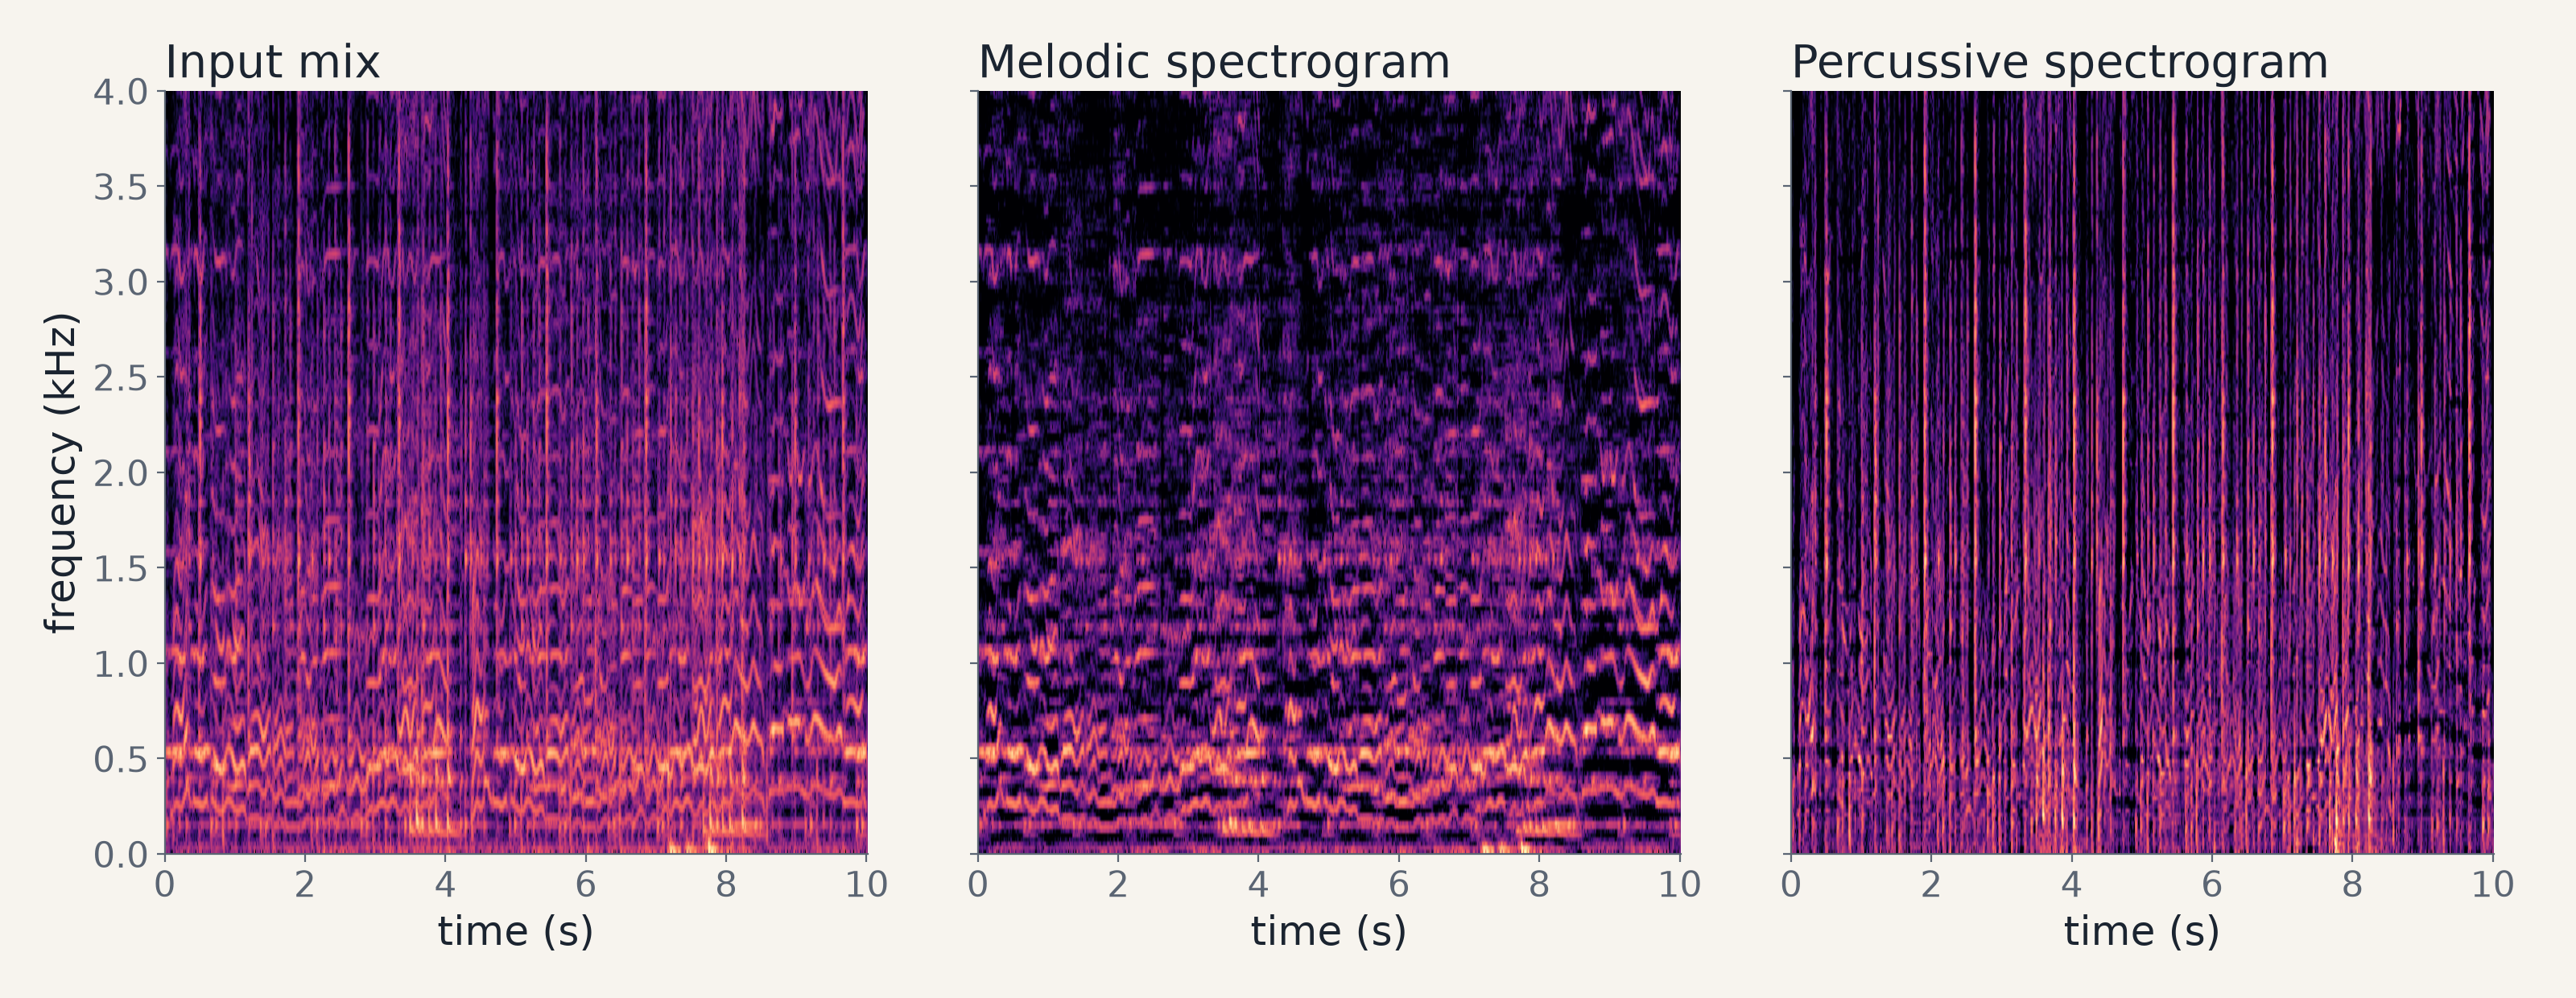
\includegraphics[width=\linewidth]{m1_hpss_spectrograms.png}
\caption{Front end on 10\,s of Carnatic ensemble audio: mixture, melodic and percussive
magnitude spectrograms, hand-written HPSS at the configured kernels (200\,ms, 500\,Hz).}
\label{fig:hpss}
\end{figure}

\section{Results}
\textbf{Front end.} Over all 37 Sanidha tracks HPSS reaches 6.84\,dB SDR on the melodic stem but
$-1.28$\,dB on the percussive one --- the baseline Milestone 2 must beat (Fig.~\ref{fig:hpss}). A
$5\times5$ kernel sweep on Concert03 shows the choice is domain-specific: the configured 200\,ms /
500\,Hz kernels give 5.07\,dB mean SDR, the best cell 5.55\,dB, and a 50\,ms time kernel loses up
to 3.4\,dB because a kernel that short cannot tell a sustained note from a stroke. Tonic
estimation is the weakest component: on 197 annotated Saraga recordings it lands within 50 cents
only 34.5\,\% of the time (median error 10 cents when correct), with 20.3\,\% taking Pa for Sa and
10.2\,\% taking Ma --- consistent with a full-mix pitch histogram dominated by the melody rather
than the drone.

\textbf{Separation} (Table~\ref{tab:results}). Fine-tuning beats the baseline by 7--9\,dB on live
recordings it never saw, but studio-to-live transfer costs about 5\,dB and is uneven: vocal
4.21\,dB, mridangam 4.83\,dB (median 8.68), violin 1.27\,dB with 41\,\% of tracks below 0\,dB,
ghatam $-8.47$\,dB. The mridangam mean is dragged down by free-rhythm pieces with no percussion:
its mic then holds only vocal and violin bleed, that bleed is scored as the reference, and the
model is penalised for correctly staying silent --- which is why its median sits 3.9\,dB above its
mean.

\begin{table}[h]
\centering
\small
\begin{tabular}{lcc}
\toprule
Method & Studio SDR & Live SDR \\
\midrule
Baseline (HPSS, mel./perc.) & 6.84 / $-1.28$ & $+1.0$ / $-2.7$ \\
Ours (re-headed HTDemucs) & \textbf{8.89} & \textbf{3.44} \\
\bottomrule
\end{tabular}
\caption{Main results. Mean SDR in dB, higher is better. ``Studio'' is the four-stem mean on
held-out Concert03, ``Live'' the three-stem mean over 168 unseen Saraga live multitracks. HPSS
cannot name instruments, so its columns group the same stems as melodic and percussive.}
\label{tab:results}
\end{table}

\textbf{Resynthesis} (Table~\ref{tab:resynth}). Mixture-phase ISTFT costs 0.8\,dB SDR against the
direct output, the price of turning directly predicted estimates into a ratio mask: where two
instruments share a bin both get the mixture's phase, and vocal and violin share the raga and
often the octave. The oracle mask sits 1.3--1.6\,dB above the predicted one on vocal, violin and
mridangam but 3.0\,dB above it on ghatam, the stem with the least training data --- better masks
would help ghatam most, while for the melodic stems the next gain must come from phase.
Griffin--Lim from random phase recovers the \emph{spectrum} almost perfectly (10.68 vs 10.78\,dB
magnitude SNR) yet scores about $-31$\,dB SDR, since BSS-Eval needs sample-level phase agreement:
the metric/perception gap in its most extreme form. The vocoder is weakest even on the
phase-blind column, and a copy-synthesis check explains why --- vocoding a \emph{clean} stem with
an all-ones mask already matches its own input only to 11.5--15.1\,dB.

\begin{table}[h]
\centering
\small
\begin{tabular}{lcc}
\toprule
Resynthesis method & SDR & mag.\ SNR \\
\midrule
HTDemucs direct waveform & 8.89 & 11.52 \\
\textbf{mask $\times$ mixture phase} & \textbf{8.08} & \textbf{10.78} \\
Griffin--Lim (random init) & $-30.81$ & 10.68 \\
Griffin--Lim (mixture init) & 6.46 & 10.88 \\
BigVGAN v2 vocoder & $-33.33$ & 8.76 \\
Oracle mask (ceiling) & 9.90 & 13.20 \\
\bottomrule
\end{tabular}
\caption{Resynthesis on held-out Concert03, mean over the four stems, dB, higher is better.
Magnitude SNR is phase-blind, the fair column for phase-reconstructing methods.}
\label{tab:resynth}
\end{table}

\textbf{Bleed removal} (Table~\ref{tab:bleed}) is what the project is really about. On studio
audio separated stems classify essentially like clean ones (94.8 vs 95.7\,\%, within 1.6 points on
every track) while the same classifier on the $-12$\,dB control collapses to 52.1\,\%: as far as
timbre is concerned, the leakage left in the separated stems is well below $-12$\,dB. An
in-domain check on held-out IMIDataset clips (97.6\,\%) confirms the measuring instrument is
sound. On \emph{live} audio separated stems beat the close microphones they were computed from,
86.3 vs 60.0\,\%, on 85--100\,\% of individual tracks.

\begin{table}[h]
\centering
\small
\begin{tabular}{lcccc}
\toprule
 & ref./mic & sep. & control & mix \\
\midrule
Studio (Concert03) & 95.7 & \textbf{94.8} & 52.1 & 22.3 \\
\quad bleed mass & 0.05 & 0.07 & 0.50 & 0.78 \\
Live (Saraga, 3 stems) & 60.0 & \textbf{86.3} & --- & 16.0 \\
\quad bleed mass & 0.42 & 0.16 & --- & 0.84 \\
\bottomrule
\end{tabular}
\caption{Bleed metric: balanced accuracy (\%), higher is better, and bleed mass, lower is better,
over 13 classes. Studio columns are clean stem / separated / clean $+$ others at $-12$\,dB /
mixture; live columns are close mic / separated / --- / sum of mics. Chance is 7.7\,\%.}
\label{tab:bleed}
\end{table}

That live gain needs splitting, because it has two possible causes: bleed on the close mic, or a
recording-domain mismatch the separator smooths over. Binning close-mic accuracy by how far a
window sits above its bleed floor separates them. Vocal and violin rise monotonically
(72.7$\rightarrow$92.8\,\% and 40.1$\rightarrow$83.6\,\%), reaching roughly where the separated
stems already sit, so for those two the gap \emph{is} bleed and separation removes it. Mridangam
instead flattens at about 48\,\% and its dominant error becomes \emph{tabla}: Saraga's live
mridangam sounds partly like tabla to this classifier even when nearly bleed-free, so its
$+47$-point gain is mostly domain adaptation and we do not claim it as bleed removal. Separating
the released master works for voice (95.3\,\%) and mridangam (86.9\,\%) but not violin (54.7\,\%,
back to close-mic level), the more honest number for separating a published recording.

\section{Discussion and limitations}
The two headline numbers disagree informatively. On live audio the separator's SDR is mediocre
(3.44\,dB) while its classifier score is excellent, and per track the two are essentially
uncorrelated ($r$ = $+0.02$ to $+0.10$). That is not noise: every Saraga reference contains room
bleed, so a separator that removes bleed \emph{cannot} match the reference and is scored down for
succeeding. SDR on live multitracks therefore cannot distinguish failure from clean separation,
and the classifier metric is the one to trust there. This is the project's main methodological
finding.

The failures are equally clear. \textbf{Ghatam} fails on live audio, has the least training data,
sits furthest from the oracle mask, and cannot even be tested by the bleed metric. \textbf{Violin}
is weak and anti-correlated with vocal per track ($r=-0.54$): Carnatic violin shadows the voice in
the same raga and often the same octave, so the shared melodic energy appears to go to one stem or
the other --- a reading we have not verified directly. \textbf{Tonic estimation} is right only a
third of the time, and the off-the-shelf \textbf{vocoder} is a negative result.

Other limits are about data. Every Saraga multitrack comes from one venue, so nothing tests a
different room. A checkpoint trained on all 37 tracks scores the same on Saraga, so the binding
constraint is Sanidha's diversity (5 concerts, little ghatam) rather than model capacity. We have
no ablation without the bleed augmentation, so we cannot prove it is what transfers. Concert03 is
not perfectly untouched: the separator never trained on it, but its epoch was \emph{selected} by
validation SDR on it, which slightly flatters the separated column. Vocal, mridangam and ghatam
come only from Sanidha, so the classifier could partly be recognising ``a Sanidha recording''. No
listening test has been run, the only fair way to judge Griffin--Lim and the vocoder. Next, by
expected value: a bleed-augmentation ablation; more ghatam and more venues; fine-tuning the
vocoder on masked estimates; and a delay-and-polarity correction so released masters can be scored
fairly.

\section{Conclusion}
Re-heading and fine-tuning a Western demixing model on 37 studio Carnatic multitracks, with bleed
simulated during training, gives a separator that transfers to live concerts it never saw and beats
a signal-processing baseline by 7--9\,dB. More useful than the SDR is the finding that SDR is the
wrong metric here: because live references are themselves bled, bleed removal had to be measured
with a downstream timbre classifier, which puts separated live stems at 86.3\,\% against 60.0\,\%
for the close microphones they came from. The remaining failures concentrate in the quietest stem
and in the instrument sharing a melodic line with the voice, pointing at corpus diversity rather
than model capacity.

\section*{Individual member contributions}
{\small
\begin{tabularx}{\linewidth}{@{}l X@{}}
\toprule
Name & Contribution \\
\midrule
Member One & STFT/HPSS front end, tonic estimation, kernel sweep and baseline; Sections 1, 3.1. \\
Member Two & HTDemucs re-heading, bleed augmentation, fine-tuning; resynthesis and vocoder; Sections 3.2--3.3, 5. \\
Member Three & Dataset loaders and de-duplication; MFCC CNN, bleed-floor rule and validation; Sections 4, 6, 7. \\
\bottomrule
\end{tabularx}}

\smallskip
\noindent All members have read this report and agree with the statement above.

\section*{Generative AI disclosure}
Claude (Anthropic, Opus-class models, via Claude Code, 2025--26) was used as a coding and writing
assistant: drafting and debugging Python across the pipeline, scripts and unit tests, and drafting
and editing this report's prose and tables, which were populated from the project's own result
JSON files. It was not used to generate data, audio or results; every number here comes from a run
of our own code on the corpora in Section~4. We have checked all such output and take full
responsibility for it. No generative model forms part of the method; the pretrained components
(HTDemucs, BigVGAN v2) are described in Section~3.

\section*{Code availability}
\noindent Code and data:\\
\url{\githuburl}\\
The repository must be public and must contain a README with instructions to reproduce the
results reported here.

\begin{thebibliography}{9}
\small
\bibitem{russell2021aima}
S.~Russell and P.~Norvig.
\newblock \emph{Artificial Intelligence: A Modern Approach}, 4th ed. Pearson, 2021.

\bibitem{sanidha2025}
Sanidha: a studio-quality multi-modal dataset of Carnatic music. \emph{arXiv:2501.06959}, 2025.

\bibitem{fitzgerald2010hpss}
D.~FitzGerald. Harmonic/percussive separation using median filtering. In \emph{Proc.\ DAFx}, 2010.

\bibitem{rouard2023htdemucs}
S.~Rouard, F.~Massa and A.~D\'efossez. Hybrid transformers for music source separation. In
\emph{Proc.\ ICASSP}, 2023.

\bibitem{hennequin2020spleeter}
R.~Hennequin et al. Spleeter: a fast and efficient music source separation tool. \emph{JOSS},
5(50):2154, 2020.

\bibitem{vincent2006bss}
E.~Vincent, R.~Gribonval and C.~F\'evotte. Performance measurement in blind audio source
separation. \emph{IEEE TASLP}, 14(4):1462--1469, 2006.

\bibitem{leroux2019sisdr}
J.~Le~Roux et al. SDR --- half-baked or well done? In \emph{Proc.\ ICASSP}, 2019.

\bibitem{griffin1984}
D.~Griffin and J.~Lim. Signal estimation from modified short-time Fourier transform. \emph{IEEE
TASSP}, 32(2):236--243, 1984.

\bibitem{lee2023bigvgan}
S.~Lee et al. BigVGAN: a universal neural vocoder with large-scale training. In \emph{Proc.\
ICLR}, 2023.

\bibitem{srinivasamurthy2021saraga}
A.~Srinivasamurthy, S.~Gulati, R.~Caro Repetto and X.~Serra. Saraga: open datasets for research on
Indian art music. \emph{Empirical Musicology Review}, 2021.
\end{thebibliography}

\end{document}
